\documentclass[aps,twocolumn,secnumarabic,balancelastpage,amsmath,amssymb,nofootinbib,floatfix]{revtex4-1}

\usepackage[colorlinks=true,linkcolor=blue]{hyperref}

\usepackage{mathexam}
\usepackage{booktabs}

%\usepackage{a4wide}
\usepackage[utf8]{inputenc}
\usepackage{amsmath}
\usepackage{amsfonts}
\usepackage{amssymb}
\usepackage{mathtools}
\usepackage[brazil]{babel}
%quebra de linha do sumário
%\usepackage[breaklinks=true]{hyperref}
%\usepackage{braket}
\usepackage{minitoc}
\usepackage{wrapfig}
\usepackage{subfigure}
\usepackage{setspace}
\usepackage{underscore}
\usepackage{indentfirst}
\usepackage{physics}

\usepackage{accents}

\usepackage{blindtext}

\usepackage{graphicx}



%\onehalfspacing


\newcommand*{\dt}[1]{%
  \accentset{\mbox{\large\bfseries .}}{#1}}
\newcommand*{\ddt}[1]{%
  \accentset{\mbox{\large\bfseries .\hspace{-0.25ex}.}}{#1}}
\newcommand*{\dddt}[1]{%
  \accentset{\mbox{\large\bfseries .\hspace{-0.25ex}.\hspace{-.20ex}}}{#1}}
\newcommand*{\dnt}[2][4]{\dt{#2}^{\tiny(#1)}}
\newcommand{\esimo}{-\text{ésimo}}
\newcommand{\esima}{-\text{ésima}}

\makeatletter
\newcommand*{\gnuplotinput}[2][1.0]{%
  \begingroup
  \let\@gnplt@input@includegraphics=\includegraphics
  \def\includegraphics##1{\@gnplt@input@includegraphics[scale=#1]{#2}}%
  \let\@gnplt@input@picture=\picture
  \def\picture{\unitlength=#1\unitlength\relax\@gnplt@input@picture}%
  \input{#2}%
  \endgroup
}
\makeatother


\makeatletter
\newcommand*{\customclear}{%
  \close@column@grid
  \cleardoublepage
  \twocolumngrid
}
\makeatother


\usepackage{listings}
\usepackage{color}

\definecolor{mygreen}{rgb}{0,0.6,0}
\definecolor{mygray}{rgb}{0.85,0.85,0.85}
\definecolor{mymauve}{rgb}{1,0.502,0}
\definecolor{numGray}{rgb}{0.3,0.3,0.3}


\lstdefinestyle{CStyle}{language=C,
  backgroundcolor=\color{mygray},   % choose the background color; you must add \usepackage{color} or \usepackage{xcolor}; should come as last argument
  basicstyle=\footnotesize,        % the size of the fonts that are used for the code
  breakatwhitespace=false,         % sets if automatic breaks should only happen at whitespace
  breaklines=true,                 % sets automatic line breaking
  captionpos=b,                    % sets the caption-position to bottom
  commentstyle=\color{mygreen},    % comment style
  deletekeywords={...},            % if you want to delete keywords from the given language
  escapeinside={\%*}{*)},          % if you want to add LaTeX within your code
  extendedchars=true,              % lets you use non-ASCII characters; for 8-bits encodings only, does not work with UTF-8
  frame=single,	                   % adds a frame around the code
  keepspaces=true,                 % keeps spaces in text, useful for keeping indentation of code (possibly needs columns=flexible)
  keywordstyle=\color{blue},       % keyword style
  language=C,                 % the language of the code
  morekeywords={*,...},            % if you want to add more keywords to the set
  numbers=left,                    % where to put the line-numbers; possible values are (none, left, right)
  numbersep=5pt,                   % how far the line-numbers are from the code
  numberstyle=\tiny\color{numGray}, % the style that is used for the line-numbers
  rulecolor=\color{black},         % if not set, the frame-color may be changed on line-breaks within not-black text (e.g. comments (green here))
  showspaces=false,                % show spaces everywhere adding particular underscores; it overrides 'showstringspaces'
  showstringspaces=false,          % underline spaces within strings only
  showtabs=false,                  % show tabs within strings adding particular underscores
  stepnumber=1,                    % the step between two line-numbers. If it's 1, each line will be numbered
  stringstyle=\color{mymauve},     % string literal style
  tabsize=2,	                   % sets default tabsize to 2 spaces
  title=\lstname                   % show the filename of files included with \lstinputlisting; also try caption instead of title
}


\lstdefinestyle{PyStyle}{language=Python,
  backgroundcolor=\color{mygray},   % choose the background color; you must add \usepackage{color} or \usepackage{xcolor}; should come as last argument
  basicstyle=\footnotesize,        % the size of the fonts that are used for the code
  breakatwhitespace=false,         % sets if automatic breaks should only happen at whitespace
  breaklines=true,                 % sets automatic line breaking
  captionpos=b,                    % sets the caption-position to bottom
  commentstyle=\color{mygreen},    % comment style
  deletekeywords={...},            % if you want to delete keywords from the given language
  escapeinside={\%*}{*)},          % if you want to add LaTeX within your code
  extendedchars=true,              % lets you use non-ASCII characters; for 8-bits encodings only, does not work with UTF-8
  frame=single,	                   % adds a frame around the code
  keepspaces=true,                 % keeps spaces in text, useful for keeping indentation of code (possibly needs columns=flexible)
  keywordstyle=\color{blue},       % keyword style
  language=Python,                 % the language of the code
  morekeywords={*,...},            % if you want to add more keywords to the set
  numbers=left,                    % where to put the line-numbers; possible values are (none, left, right)
  numbersep=5pt,                   % how far the line-numbers are from the code
  numberstyle=\tiny\color{numGray}, % the style that is used for the line-numbers
  rulecolor=\color{black},         % if not set, the frame-color may be changed on line-breaks within not-black text (e.g. comments (green here))
  showspaces=false,                % show spaces everywhere adding particular underscores; it overrides 'showstringspaces'
  showstringspaces=false,          % underline spaces within strings only
  showtabs=false,                  % show tabs within strings adding particular underscores
  stepnumber=1,                    % the step between two line-numbers. If it's 1, each line will be numbered
  stringstyle=\color{mymauve},     % string literal style
  tabsize=2,	                   % sets default tabsize to 2 spaces
  title=\lstname                   % show the filename of files included with \lstinputlisting; also try caption instead of title
}

\newenvironment{tk3} {
\tikzstyle{loop} = [regular polygon, regular polygon sides=6, shape aspect=0.3, minimum width=1cm, minimum height=1cm, draw,scale=.7, align=center, text width=0.9	cm, fill = blue!15]

\tikzstyle{startstop} = [rectangle, rounded corners, minimum width=3cm, minimum height=.7cm,text centered, draw=black, fill=red!30, text width = 6cm]

\tikzstyle{process} = [rectangle, minimum width=3cm, minimum height=1cm, text centered, draw=black, fill=orange!30, text width = 4cm]

\tikzstyle{processSmall} = [rectangle, minimum width=1cm, minimum height=1cm, text centered, draw=black, fill=orange!30, text width = 2cm]

\tikzstyle{decision} = [diamond, draw, fill=yellow!30,
    text width=4.5em, text badly centered, node distance=3cm, inner sep=0pt]

\tikzstyle{line} = [draw, -latex']

\tikzstyle{cloud} = [draw, ellipse,fill=red!20, node distance=3cm, minimum height=2em, text width = 4cm]

\tikzstyle{io} = [trapezium, trapezium left angle=70, trapezium right angle=-70, text centered, text width = 3.5cm, minimum height=1cm, minimum width=2cm, draw=black, fill=blue!30]

\tikzstyle{arrow} = [thick,->,>=stealth]
\tikzstyle{line} = [draw, -latex']
} {  }

\begin{document}
  \begin{center}
    \LARGE \textbf{Física Computacional} \\
    \Large \textbf{Tarefa 7 - Questão 3} \\
    \large Alex Enrique Crispim
  \end{center}

  O método de Runge-Kutta de quarta ordem segue uma ideia semelhante ao caso feito para a questão 2, porém tomando a expansão até quarta ordem.

  Seguindo o mesmo procedimento, com um pouco mais de álgebra, chegamos às seguintes equações:
  \begin{equation}
    x(t+ h) = x(t) + \frac{1}{6} \qty(K_1 + 2K_2 + 2K_3 + K_4).
    \label{eq:1}
  \end{equation}
  \begin{equation}
    \begin{cases}
      K_1 &= h f(t, x) , \\
      K_2 &= h f(t + \frac{1}{2} h, x + \frac{1}{2} K_1), \\
      K_3 &= h f(t + \frac{1}{2} h, x + \frac{1}{2} K_2), \\
      K_4 &= h f(t + h, x + K_3).
    \end{cases}
    \label{eq:2}
  \end{equation}

  O algoritmo para o método Runge-Kutta-4 é praticamente o mesmo para o Runge-Kutta-2, como mostrado abaixo.
  \begin{figure}[h]
    \center
    \begin{tk3}
    \begin{tikzpicture}[node distance = 15 mm, auto]
      \node (start) [startstop] {Algoritmo de Runge-Kutta de quarta ordem};
      \node (initializing) [process, below of = start] {Inicializa $f(t, x)$, $t  \leftarrow t_0$, $t_f$, $x_0$ e $h$};
      \node (CalcKs) [process, below of = initializing] {Calcula $K_1$, $K_2$, $K_3$ e $K_4$ via (\ref{eq:2}).};
      \node (newX) [process, below of = CalcKs] {$x_{i+1} = x_i + \frac{1}{2} (K_1 + 2K_2 + 2K_3 + K_4)$; (eq. \ref{eq:1}) \\ $t \leftarrow t + h$};
      \node (dec) [decision, right of = newX, xshift = 8mm] {$(t > t_f)$?};
      \node (printX) [io, below of = newX] {Imprime \texttt{x[]} em função de $t$.};
      \node (stop) [startstop, below of = printX] {Finalizado};

      \draw [arrow] (start) -- (initializing);
      \draw [arrow] (initializing) -- (CalcKs);
      \draw [arrow] (CalcKs) -- (newX);
      \draw [arrow] (newX) -- (dec);
      \path [line]  (dec) -- (3.8,-3.0) -- node [anchor = south]{não} (CalcKs);
      \path [line]  (dec) -- (3.8,-6.0) -- node [anchor = north]{sim} (printX);
      \draw [arrow] (printX) -- (stop);
    \end{tikzpicture}
    \end{tk3}
    \caption{Algoritmo de RK4 para a solução de EDO's}
  \end{figure}

  Uma implementação do algoritmo RK4 pode ser encontrado na pasta \textit{question 3} do endereço: \url{https://github.com/AlexEnrique/comp-physics-pratice7}.

  É importante mencionar que, como o próprio nome do método sugere, o algoritmo RK4 tem seu erro de quinta ordem em $h$ (a série é truncada em quarta ordem). Isso significa uma convergência muito mais rápida em comparação com RK2 (Runge-Kutta de segunda ordem). Como exemplo, considere $h = 10^{-2}$. Para RK2 temos um erro de ordem $\order{10^{-6}}$, enquanto que para RK4 o erro é $\order{10^{-10}}$.

  O grande problema com o algoritmo RK4 se dá quando a EDO envolvida é tal que as soluções se distanciam entre si conforme a variável $t$ cresce. Por exemplo, para a EDO $x^\prime = 10x + 11 t - 5t^2 - 1 $, com $x(0) = 0$, o método RK4 nos dá um resultado errado. As figuras abaixo mostram as soluções exatas (vermelho) e via RK4 para a EDO acima.
  \begin{figure}[h]
    \center
    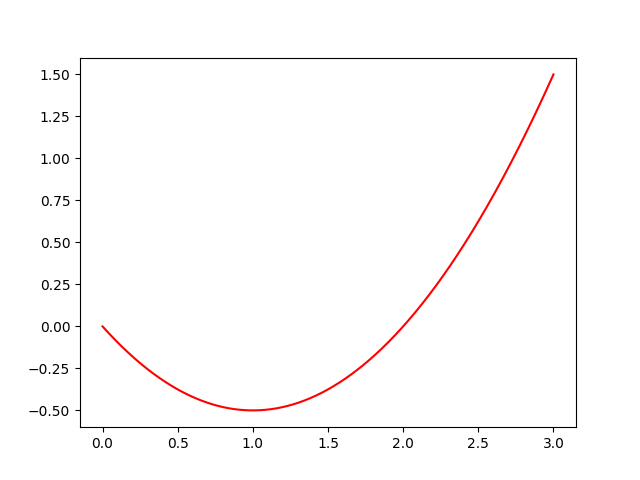
\includegraphics[scale = .45]{Figure1}
    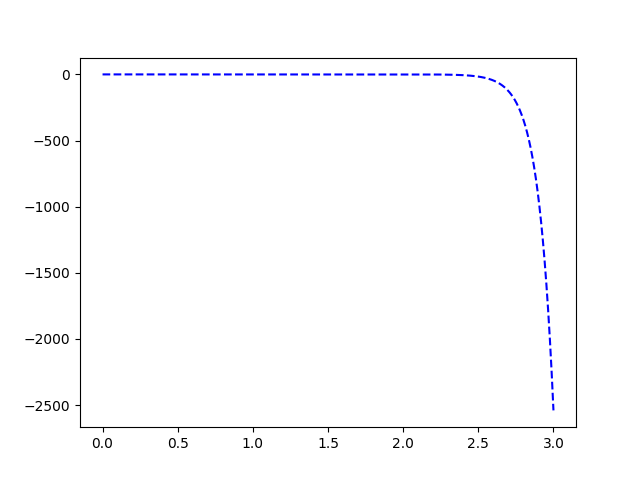
\includegraphics[scale = .45]{Figure2}
  \end{figure}

  O problema se deve ao fato de que, uma variação $h$ nas condições iniciais leva a uma variação muito grande dos valores esperados para a função. Considere por exemplo a EDO dada por
  \begin{equation*}
    x^\prime = f(t, x), \\
    x(0) = s.
  \end{equation*}

  Se trocamos $s$ por $s+h$ (o que é induzido, por exemplo, por um erro de arredondamento), devemos considerar a função $x(t)$ como a depender do parâmetro $s$ da forma de uma variável, escrevendo $x(t, s)$ no lugar. Podemos expandir $x(t, s+h)$ em Taylor da seguinte forma
  \begin{equation*}
    x(t, s+h) = x(t,s) + h \pdv{s} x(t, s) + \order{h^2}.
  \end{equation*}

  A divergência entre a função esperada $x(t, s)$ e $x(t, s+h)$ pode ser escrita como
  \begin{equation*}
    \lim_{t \to \infty} \abs{x(t, s+h) - x(t,s)} = \infty \Leftrightarrow \lim_{t \to \infty} \abs{\pdv{s} x(t, s)} = \infty
  \end{equation*}

  Para calcular a derivada parcial de $x$ com relação a $s$, usamos o seguinte procedimento:
  \begin{equation*}
    \pdv{t} \pdv{s} x(t, s) = \pdv{s} \pdv{t} x(t,s) = f_x(t, x(t,s)) \pdv{s} x(t,s) + f_t(t, x(t,s)) \pdv{t}{s},
  \end{equation*}
  como uma variação em $t$ não depende de uma variação em $s$, $\pdv{t}{s} = 0$ e fazendo $u(t) = \pdv{s} x(t,s)$ e $q(t) = f_x(t, x(t,s))$, obtemos a seguinte EDO, da relação anterior:
  \begin{equation*}
    u^\prime = q u ,
  \end{equation*}
  cuja solução é $u = c e^{Q(t)}$, com
  \begin{equation*}
    Q(t) = \int_a^t \dd{\theta} q(\theta).
  \end{equation*}

  A divergência do limite de $\abs{\pdv*{x}{s}}$ se dá então pela divergência de $Q(t)$ (pois leva a diergir ($u$)).

  Se $Q$ for uma função positiva e limitada inferiormente por um valor maior do que zero, é fácil ver que a função diverge:
  \begin{equation*}
    Q(t) = \int_a^t \dd{\theta} q(\theta) > \int_a^t \delta \dd{\theta} = \delta (t-a) \xrightarrow[t \to \infty]{} \infty.
  \end{equation*}

  A conclusão final é: a solução diverge se $f_x > \delta$ e converge quando $f_x < - \delta$, com $\delta > 0$.

  Para a EDO fornecida para as questões 1, 2 e 3, $f(t, x) = - x^3 + \sin(t)$ e, logo, $f_x = -x^2 \leq 0, \forall x$, enquando que a EDO mal-comportada acima leva à $f_x = 10 > 0$, divergindo do valor real.

\end{document}
